%%%%%%%%%%%%%%%%%%%%%%%%%%%%%%%%%%%%%%%%%%%%%%%%%%%%%%%%%%%%%%%%%%%%%%%%%%%%%%%%%%%%%%%%%%%%%%%%%%%%%%%%%%
%%%   %%%%
%%%%%%%%%%%%%%%%%%%%%%%%%%%%%%%%%%%%%%%%%%%%%%%%%%%%%%%%%%%%%%%%%%%%%%%%%%%%%%%%%%%%%%%%%%%%%%%%%%%%%%%%%%%

\documentclass{sig-alternate}

\usepackage[utf8]{inputenc}
\usepackage{amssymb}
\setcounter{tocdepth}{3}
\usepackage{graphicx}
\usepackage{tabularx}
\usepackage{url}
\usepackage{listings}
\usepackage{subfigure}
\usepackage{algorithmic}
\usepackage{algorithm}
\usepackage{verbatim}

%\newcommand{\keywords}[1]{\par\addvspace\baselineskip
%\noindent\keywordname\enspace\ignorespaces#1}

% todo macro
\usepackage{color}
\newtheorem{deflda}{Axiom}
\newcommand{\todo}[1]{\noindent\textcolor{red}{{\bf \{TODO}: #1{\bf \}}}}
\newcommand{\neon}{NeOn }
\newcommand{\protege}{Prot{\'e}g{\'e} }



%%%%%%%%%%%%%%%%%%%%%%%%%%%%%%%
%%%  Beginning of document  %%%
%%%%%%%%%%%%%%%%%%%%%%%%%%%%%%%

\begin{document}

% first the title is needed
% --- ACM copyright metadata here ---
%\conferenceinfo{SEM}{14, September 04 - 05 2014, Leipzig, AA, Germany}
%\CopyrightYear{2015}
%\crdata{978-1-4503-2927-9/14/09.}


%\title{How to access and reuse ontologies in real-world scenarios}
\title{Towards a Linked Dataset for French Districts Evolution}

\numberofauthors{1}
\author{
% 1st. author
\alignauthor Ghislain Auguste Atemezing\\
       \affaddr{MONDECA}\\
       \affaddr{35 boulevard Strasbourg, Paris, France}\\
       \email{\small{ghislain.atemezing@mondeca.com}}
% 3rd author
  \alignauthor Nuria Garc{\'i}a-Santa\\
       \affaddr{Expert System Iberia}\\
       \affaddr{Campo de las Naciones, Madrid, Spain.}\\
       \email{\small{ngarcia@expertsystem.com}}
% 2nd. author
\alignauthor Boris Villaz{\'o}n-Terrazas\\
       \affaddr{Expert System Iberia}\\
       \affaddr{Campo de las Naciones, Madrid, Spain.}\\
       \email{\small{bvillazon@expertsystem.com}}       
}

\maketitle


%%%%%%%%%%%%%%%%%%
%%%  Abstract  %%%
%%%%%%%%%%%%%%%%%%

\begin{abstract}
This paper provides a real-world scenario of combining heterogeneous datasets in plain text and shape files to create a dataset in RDF of the French districts evolution since 1790. We use two different datasets (1) a shape file containing polygons from the French Geographic Institute (IGN) and (2) a text file containing names of districts and events occurred at a certain time (fusion, merging, etc) with other entities from the National Statistics Institute (INSEE).  

This work explores the use of semantic technologies to combine heterogeneous datasets (text and shape) for creating an RDF dataset explaining the geo-dynamic evolution of districts occurred since the French revolution. The resulting dataset reuses standard vocabularies for topographic entities, geometries, provenance and time. The expected outcome of the dataset is to interlink with other historical facts and build innovative applications consuming the dataset.
%\keywords{ontology engineering, ontology reuse, LOV, Prot{\'e}g{\'e}, Plugin} 
\end{abstract}

% Categories for the papers.
%\todo{Replace with the categories provided by Nuria}
%\category{M}{Knowledge Management}
%\category{M.1}{Knowledge engineering methodologies}
%\category{M.1}{Knowledge engineering methodologies}
%\category{M.8.}{Knowledge Reuse}
\category{H.4}{Information Systems Applications}{Miscellaneous}
\category{H.3.5}{Online Information Services}{Data sharing}[Web-based services]

\terms{geospatial data, RDF modeling, Linked Data}

\keywords{geodata, Linked dataset, aligning heterogeneous data}


%%%%%%%%%%%%%%%%%%%%%%%%%
%%%  1. Introduction  %%%
%%%%%%%%%%%%%%%%%%%%%%%%%


\section{Introduction}\label{sec:introduction}
%\todo{we have to extend this Related work}

So far, Linked Data principles and practices are being adopted by an increasing number of data providers, getting as result a global data space on the Web containing hundreds of LOD datasets \cite{Heath_Bizer_2011}. There are already several guidelines for generating, publishing, interlinking, and consuming Linked Data \cite{Heath_Bizer_2011}. An important task, within the generation process, is to build the vocabulary to be used for modelling the domain of the data sources, and the common recommendation is to reuse as much as possible available vocabularies \cite{Heath_Bizer_2011,hyland14}. This reuse approach speeds up the vocabulary development, and therefore, publishers will save time, efforts, and resources. 

There are research efforts, like the NeOn Methodology \cite{suarezfigueroa2012ontology}, the Best Practices for Publishing Linked Data - W3C Working Group Note \cite{hyland14}, and the work proposed by Lonsdale et al. \cite{Lonsdale2010318}. However, at the time of writing we have not found specific and detailed guidelines that describe how to reuse available vocabularies at fine granularity level,i.e., reusing specific classes and properties. Our claim is that this difficulty in how to reuse vocabularies at fine grained level is one of major barriers to the reuse of vocabularies on the Web and in consequence to deployment of Linked Data.

Moreover, the recent success of Linked Open Vocabularies (LOV\footnote{\url{http://lov.okfn.org/dataset/lov/}}) as a central point for curated catalog of ontologies is helping to convey on best practices to publish vocabularies on the Web, as well as to help in the Data publication activity on the Web. LOV comes with many features, such as an API, a search function and a SPARQL endpoint.

In this paper we propose a set of guidelines for this task, and provide technological support by means of a plugin for \protege, which is one of the popular frameworks for developing ontologies in a variety of formats including OWL, and RDF(S). It is backed by a strong community of developers and users in many domains. One success on \protege also depends on the availability to extend the core framework adding new functionalities by means of plug-ins. In addition, we propose to explore, design and implement a plug-in of LOV in \protege for easing the development of ontologies by reusing existing vocabularies at fine grained level. The tool helps to improve the modeling and reuse of ontologies used in the LOD cloud.

%, by providing the following features in Prot{\'e}g{\'e}:
%\begin{itemize}
%\item Import easily vocabularies from LOV into \protege. 
%\item Propose to the user a list of candidate vocabularies in LOV matching the term
%\item Have an updating mechanism (synchronization) to LOV catalog
%\item Check if a new vocabulary created in \protege satisfied the LOV recommendations \cite{pybernard12}
%\item Suggest to LOV a new created vocabulary within \protege.
%\end{itemize}

%This paper presents \protege, a first implementation of the LOV realized as a plugin for the ontology editor \protege. 





  





%%%%%%%%%%%%%%%%%%%%%%%%%%%%%%%%%%%%%%%%%%%%%%%%%%
%%%  2. Related work  %%%
%%%%%%%%%%%%%%%%%%%%%%%%%%%%%%%%%%%%%%%%%%%%%%%%%%

\section{Related Work}\label{sec:soa}
%Show here some work related to plugin for helping in ontology development:Neon and other
%\todo{target to guidelines}
\todo{I suggest to move this related work at the end}
In the literature there exist many attempts to advise vocabulary publishers on the importance of reusing terms, as indicated in \cite{janowicz2014five,jimenez2008}. However, to the best of our knowledge there are not guidelines to help vocabulary practitioners to reuse vocabularies in real-world scenario, and considering specific ontology/vocabulary elements. 

In the W3C Government Linked Data best practice document \cite{hyland14}, reusing vocabularies is recommended by providing to stakeholders a basic checklist when using or extending a vocabulary. It gives general guidance to follow before publishing the vocabulary, not guidance during the creation of the vocabulary. Our proposal is to guide the users during the implementation process.

Recently, Janowicz et al. have proposed a 5 stars rating for Linked (Open) Data vocabulary use to ``encourage data owners, engineers and practitioners to publish and use vocabularies on the Web'' \cite{janowicz2014five}. They make it clear that the rating do not refer to the quality of the vocabularies. In the definition of the rating system, the third star is given to a vocabulary linked to other vocabularies by means of explicit alignments and import of external vocabularies. Our guidelines make it easier to vocabulary publishers to obtain at least 3-star vocabularies.

Other initiatives similar to the tool we have developed can be found in the literature but not currently maintained. The BioPortal Reference Plugin\footnote{\url{http://protegewiki.stanford.edu/wiki/BioPortal_Reference_Plugin}} allows the user to insert into the ontology references to external ontologies and terminologies stored in BioPortal\footnote{\url{http://bioportal.bioontology.org/}}. The plugin allows to generate external reference of a selected term. Additionally, the BioPortal Import Plugin\footnote{\url{http://protegewiki.stanford.edu/wiki/BioPortal_Import_Plugin}} allows users to import classes from external ontologies stored in the BioPortal ontology repository. The user can import entire trees of classes with a desired depth and choose which properties to import for each class. However, those plugins work only with \protege 3.x releases and are not ported yet to recent versions. 

Most closely related to the {\protege}LOV plugin are approaches that use semantic search engine to support the process of editing an ontology and make large scale knowledge reuse automatically integrated in the tool. An example is the Watson Plugin \cite{neonguide2008} for the \neon Toolkit \cite{haase2008neon}, a plugin supporting the \neon life-cycle management using the Watson \cite{d2007watson} APIs\footnote{\url{http://watson.kmi.open.ac.uk/WS_and_API.html}}.However the similar plugin for Protege\footnote{\url{http://protegewiki.stanford.edu/wiki/Watson_Search_Preview}} is just a proof of concept rather than a real plugin.

 



\section{Legacy Datasets}
\label{sec:legacy}
%\todo{We have to improve this section- add a picture for workflow}
%\todo{Boris will do it}


We obtained the dataset from two different sources: the text file from INSEE website in text file and the shape file from the output of an ANR project. 

\subsection{Text file with districts events}
The text from INSEE contains information of different modifications occurred in France from 1930 until 2013. Each line represents a piece of information with an INSEE code (5 digit), the date in the form DD/MM/YYYY and a string describing the event. For example, `` 38205	09/05/1947	Lans devient Lans-en-Vercors'' states that on the 9th May, 1947 Lans with INSEE code 38205 became ``Lans-en-Vercors''. 


\subsection{Shape file with geometries}
We obtained a license copy of the shape file with the ANR project Geopeuple\footnote{\url{http://geopeuple.ign.fr/}}

%In this section, we describe the workflow for reusing available vocabulary terms when building ontologies based on an existing catalogue of vocabularies. Recall that we do not specify which will be the expressivity of the resulting ontology. We foresee that the resulting ontology is likely to be a lightweight ontology. However the data publisher is responsible for adding more semantics when reusing existing vocabulary terms. Figure \ref{fig:workflow} depicts the proposed workflow. 

\begin{figure}
\centering
%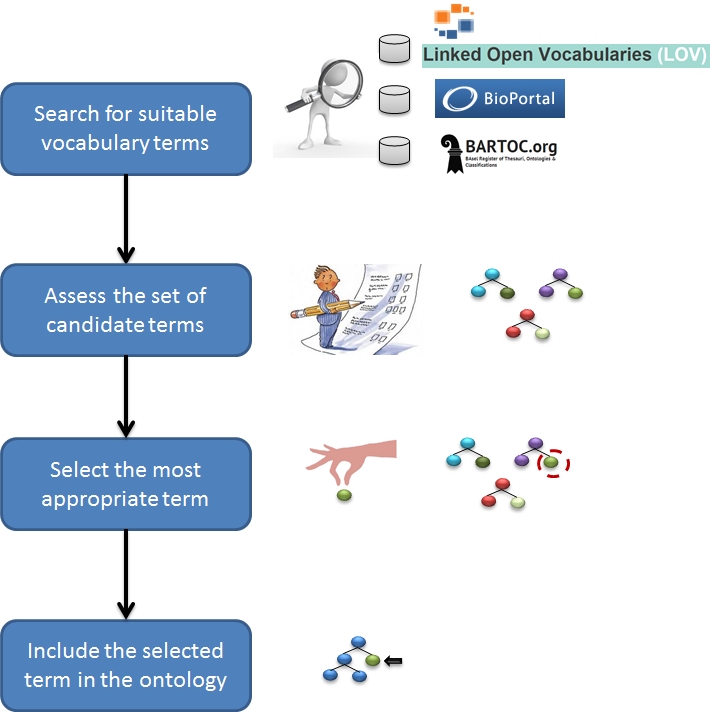
\includegraphics[scale=0.5]{./img/process}
\caption{Workflow for reusing available terms when building ontologies}
\label{fig:workflow}
\end{figure}


\begin{comment}
\subsection{Use case scenario: lobid vocabulary}
\label{lobid vocabulary}
Looking at the evolution of some vocabularies with highest changes since their release in LOV,\texttt{lobid} vocabulary is the winner with 16 modifications. The \texttt{lobid} vocabulary\footnote{\url{http://purl.org/lobid/lv}} is a vocabulary designed for the  linking open bibliographic data services. The ontology was first published on 2012-03-02 with only two properties, a minimal metadata information and labels in English. Since then, there have been 15 different versions and the current version (version of 2015-02-09) of the ontology contains 8 classes and 16 properties. Based on the different changes occurred during the on-going development of the lobid vocabulary, vocabulary changes can be grouped in two categories:
\begin{itemize}
\item Editorial changes (EDc) are the ones related with labels and comments translations, typos fixed. Those changes don't affect the structure of the vocabulary.
\item Semantic changes (SMc) are related with modifying the structure of the vocabulary, by either adding new axioms, new classes and properties.
\end{itemize}

Furthermore, the semantic changes can be broken down in four categories related to the main parts of a vocabulary, that are metadata, classes, properties and axioms. Thus we can group them as follows:

\begin{itemize}
\item Metadata changes (MTc), when the changes are related with the metadata section of the vocabulary. E.g., adding provenance information, license, publishers and creators data.
\item Property changes (PPc), when updating the vocabulary 
\item Classes changes (CLc), such as the creation of named classes.
\item Axioms changes (AXc) for updates using some axioms for restrictions in or the creation of anonymous classes. 

\end{itemize}

Table \ref{tab:lobid} summarizes the number of changes for the lobid vocabulary. In  a total of 20 changes, only 2 are editorial changes and each time accompanied with a semantic change in the corresponding version.
\texttt{lobid} vocabulary is a good example of reusing existing terms where the definition of all the classes are ``subclassing'' of three existing vocabularies: \texttt{dct}, \texttt{bibo} and \texttt{archives}\footnote{\url{http://data.archiveshub.ac.uk/def/}}.  

\begin{table}[!htb]
\centering{

\begin{tabular}{lccccc}
\hline
 \textbf{Changes} & EDc & MTc & PPc & CLc & AXc \\ \hline
  Numbers & 2 & 4 & 8 & 3 & 3 \\
 
 \hline
\end{tabular}
\caption{Changes observed in the lobid vocabulary since its release in 2012. }
\label{tab:lobid}
}
\end{table}

\end{comment}


%\subsection{Workflow on Reusing Terms}
In a nutshell, the activity of building vocabularies by reusing available vocabulary terms consists of the following tasks:

\begin{itemize}
	\item Search for suitable vocabulary terms to reuse from any vocabulary repository, such as BioPortal\footnote{\url{http://bioportal.bioontology.org/}}, LOV\footnote{\url{http://lov.okfn.org/}}, Bartoc.org\footnote{\url{http://bartoc.org}}, etc. The search should be conducted by using the terms of the application domain.
	\item Assess the set of candidate terms from the vocabulary repository. The goal of this task is to find out if the candidate terms are useful and relevant for the ontology being built. For this purpose we can rely on metrics provided by the vocabulary repository. In the particular case of LOV, the results include a score related to their ``importance'' in the corpus for each term retrieved. For every vocabulary in the LOV, terms (classes, properties, datatypes, instances) are indexed and a full text search feature is offered\footnote{\url{http://lov.okfn.org/dataset/lov/terms}}. The Linked Open Vocabularies search engine ranking algorithm takes  into account the popularity of the term within the LOV ecosystem and most importantly assigned a different score depending on which label property a searched term matched~\cite{vandenbusschelov}.		
	\item Select the most appropriate term taking into account the assessment task. To distinguish between those candidate terms which are the most suitable, we propose to use the following criteria (i) the stability of the URI namespace, (ii) the trustworthiness of the publisher of the vocabulary and (iii) the presence or absence of a community using the vocabulary. With respect to LOV repository we can also rely on the score of terms.
	\item Include the selected term in the ontology that has being developed. There are at least three alternatives in this case 
	\begin{itemize}
		\item Include the selected term and use it directly, i.e., as it is, in the local ontology by defining local axioms to or from that term in the local ontology.
		\item Include the selected term, create a local term, and define the {\tt rdfs:subClassOf} or {\tt rdfs:subPropertyOf} axiom to relate both terms.
		\item Include the selected term, create a local term, and define the {\tt owl:equivalentClass} or \\ {\tt owl:equivalentProperty} axiom to relate both terms. 				
	\end{itemize}
\end{itemize}

It is worth mentioning the following considerations
\begin{itemize}
	\item We want to promote a ``responsible'' reutilization, i.e., if the user already found something interesting in a particular vocabulary, the user would probably like to dig a little bit more on it, suggesting other terms in it, before jumping somewhere else.
	\item We want to keep consistency of reused terms . Therefore, it would be necessary to (1) check and update the domain/range of the selected terms; (2) change cardinalities; and (3) add some restrictions.
	\item We want to bring as many knowledge as possible from the reused term, e.g., for a particular property it would be necessary to check if a inverse property exists and import it as well.
\end{itemize} 


%%%%%%%%%%%%%%%%%%%%%%%%%%%%%%%%%%%%%%%%%%%%%%%%%%%
%%%  3.LOV APIs Description  %%%
%%%%%%%%%%%%%%%%%%%%%%%%%%%%%%%%%%%%%%%%%%%%%%%%%%%
%\vspace{-3mm}
%\section{Linked Open Vocabulaires (LOV)}\label{sec:lov}

\section{RDF Dataset Creation}
\label{sec:creation}
Include the process of creating RDF dataset


The intended purpose of the LOV \cite{vandenbusschelov} is to help users to find and reuse terms of vocabularies in Linked Open Data. For achieving that purpose, the LOV gives access to vocabularies metadata and terms using programmatic access with APIs.  
LOV\footnote{\url{http://lov.okfn.org/dataset/lov/}} catalogue is a hub of curated vocabularies used in the Linked Open Data Cloud, as well as other vocabularies suggested by users for their reuse. 
Some of the three main features of the LOV are for: (1) searching ontologies according to their scope, (2) assessing ontologies by providing a score for each term retrieved by a keyword search and (3) interconnecting ontologies using VOAF vocabulary\footnote{\url{http://lov.okfn.org/vocab/voaf}}.
The search function uses an algorithm based on the term
popularity in LOD and in the LOV ecosystem. The matched resource set for each term should be the value of the a) {\tt rdfs:label} b) {\tt rdfs:comment}, or c) {\tt rdfs:description} property.

For every vocabulary in the LOV, terms (classes, properties, datatypes, instances) are indexed and a full text search feature is offered\footnote{\url{http://lov.okfn.org/dataset/lov/terms}}. The Linked Open Vocabularies search engine ranking algorithm takes into account the popularity of the term within the LOV ecosystem and most importantly assigned a different score depending on which label property a searched term matched. For example, a term matching a value for the property \url{rdfs:label} will have a higher score than if it matches a value for the property \url{dcterms:comment}.

%\begin{enumerate}
%\item Searching ontologies: It is the main LOV's feature is the search of vocabulary terms. These vocabularies are categorized within LOV according to the domain they address. In this way, LOV contributes to ontology search by means of (a) keyword search and (b) domain browsing.
% \item Assessing ontologies: LOV provides a score for each term retrieved by a keyword search. This score can be used during the assessment stage.
% \item Interconnecting ontologies: In LOV, vocabularies rely on each other in seven different ways. These relationships are explicitly stated using VOAF vocabulary\footnote{\url{http://lov.okfn.org/vocab/voaf}}. 
%\end{enumerate}

Futhermore, the LOV APIs give a remote access to the many functions of LOV through a set of RESTful services\footnote{\url{http://lov.okfn.org/dataset/lov/apidoc/}}. %The basic design requirements for these APIs is that they should allow applications to get access to the very same information humans do via the User Interfaces. More precisely the
The APIs give access through three different type of services related to: (1) vocabulary terms (classes, properties, datatypes and instances), (2) vocabulary browsing and (3) ontology's creators. 

%\begin{enumerate} 
%	\item vocabulary terms (classes, properties, datatypes and instances) providing functions to query the LOV search engine, with autocompletion features;
%	\item vocabulary browsing, in which a client can get access to the current list of vocabularies contained in the LOV catalogue and search for vocabularies for further purpose;
%	\item agents, or the ontology's creators, contributors or organizations. It also contains the search with autocompletion of an agent.
%	\end{enumerate}

%to continue 





%%%%%%%%%%%%%%%%%%%%%%%%%%%%%%%%%%%%%%%%%%%%%%%%%%%
%%%  4.ProtegeLOV Description  %%%
%%%%%%%%%%%%%%%%%%%%%%%%%%%%%%%%%%%%%%%%%%%%%%%%%%%
%\vspace{-3mm}
%\section{Prot{\'e}g{\'e}LOV}\label{sec:classification}
%\input{plugin-core}


%%%%%%%%%%%%%%%%%%%%%%%%%%%%%%%%%%%%%%%
%%%  5. Conclusion and Future Work  %%%
%%%%%%%%%%%%%%%%%%%%%%%%%%%%%%%%%%%%%%%

%\section{Evaluation}\label{sec:conclusion}
%This section presents the experiment that has been carried out and with two main objectives (1)  evaluating the understandability, applicability and usability of the methodological contributions; and (2) evaluating the usability of the Prot{\'e}g{\'e}LOV plug in.
\vspace{1mm}
\subsection{Experiment Settings}
For this experiment, fifteen ontology engineers built a small ontology by following the methodological guidelines provided here\footnote{\url{http://labs.mondeca.com/protolov/method.html}} and using the Prot{\'e}g{\'e}LOV plugin\footnote{\url{http://labs.mondeca.com/protolov/}}. After the interaction with the methodological guidelines and the plugin the participants filled in a questionnaire available here \footnote{\url{https://goo.gl/vMzHU2}}.
\vspace{1mm}
\subsection{Finding and observations}
For this preliminary evaluation we keep the number of evaluators low. The results indicate that while the tool needs some minor improvements, the majority of the evaluators still consider the tool to be useful. Moreover, most of the participants provided very good feedback about the proposed methodological guidelines.


%Finally, it is worth mentioning we have presented our plugin as demo papperused two pools for evaluating the tools: 16 experts in ontology modeling selected randomly and spontaneous visitors that came to our booth during the last ESWC 2015 in Portoroz. It has been difficult to receive the 
 

\begin{comment}
\subsection{Other evaluation?}

We have conducted an initial user driven evaluation of the tool. For this preliminary evaluation we keep the number of evaluators low; seven ontology engineers used our plugin and gave us an insight on their experience by filling in a questionnaire \footnote{\url{http://goo.gl/H4YgBJ}}. The results indicate that while the tool needs some minor improvements, the majority of the evaluators still consider the tool to be useful.
\end{comment}
\vspace{3mm}
\section{Conclusions and Future Work}
\label{sec:conclusions}
In this paper we have presented (1) initial guidelines that describe how to reuse available vocabularies at fine-grained level, i.e., by reusing specific classes and properties, and (2) a tool that provides technological support by means of a plugin for \protege that access LOV API. Moreover, we have presented the first evaluation we have performed for our guidelines and their technological support.


As future work we plan to evaluate the guidelines and tool with a large set of users. Also, we plan to include access to other respoitories, e.g., Bioportal and Bartoc. Finally, we plan to develop a plugin with the same functionalities for other tools, such as  Web-\protege\footnote{\url{http://webprotege.stanford.edu/}} and TopBraid composer\footnote{\url{http://www.topquadrant.com/tools/ide-topbraid-composer-maestro-edition/}}.


%During the demonstration we will show to potential users how to install the plugin and how to quickly build ontologies by reusing terms from LOV repository in \protege.





%%%%%%%%%%%%%%%%%%%%%%%%%
%%%  Acknowledgments  %%%
%%%%%%%%%%%%%%%%%%%%%%%%%
\vspace{1mm}
\paragraph{\textbf{Acknowledgments.}} %\label{sec:acknowledgments}
Thanks to Pierre-Yves and the LOV team for maintaining the LOV catalog and the API access. This work has been supported by the KDrive Project.
% More acknowledgments here
%\vspace{-3mm}

\bibliographystyle{abbrv}
%\nocite{*}
\bibliography{gir15}
\balancecolumns
\end{document}
